\section{Backend}
%TODO: @Joshua

\subsection{Aufbau}

Der Aufbau der Serverapplikation orientiert sich am Konzept der Onion-Architecture.
In Onion Architecture wird die Applikation in Layer aufgeteilt.

\begin{figure}[h]
    \centering
    \begin{minipage}[b]{0.4\textwidth}
        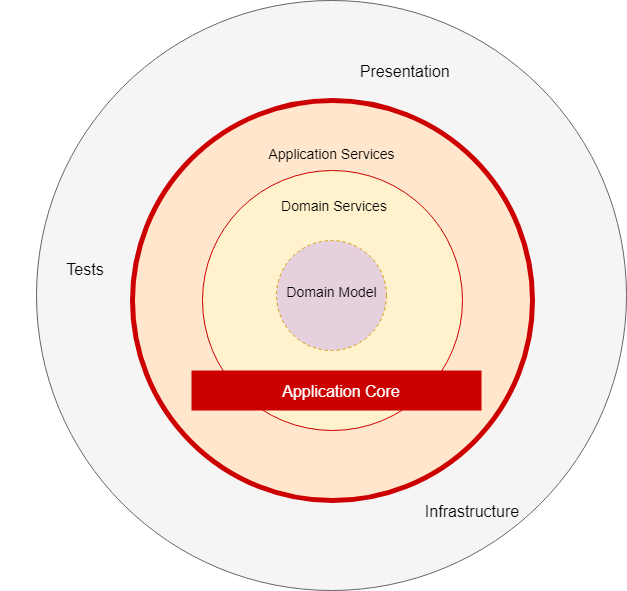
\includegraphics[width=\textwidth]{graphics/thinktocode-onion}
        \caption{Onion Architecture}
    \end{minipage}
\end{figure}

Um zu garantieren, dass keine ungewollten Abhängigkeiten zwischen Layern bestehen, können die Layer in eigene Module verpackt und Abhängigkeiten über Interfaces abstrahiert werden.
Dies erhöht jedoch die interne Komplexität der Applikation.
Die Umsetzung wird aufgrund der geringen Projektgrösse deshalb nicht in unabhängigen Modulen realisiert, sondern über die Package Struktur gelöst.
Bei der Implementation wird dabei konsequent darauf geachtet, die einzelnen Layer so zu halten das diese als eigenständige Module extrahiert werden können.
Für die Verwaltung der Komponenten der Serverapplikation wird folgende Packagestruktur definiert:

\begin{figure}[h]
    \centering
    \begin{minipage}[b]{0.9\textwidth}
        \dirtree{%
            .1 ch.fhnw.woweb.teamdocumentserver.
            .2 config.
            .2 domain.
            .2 persistence.
            .2 service.
            .2 web.
        }
        \caption{Package Struktur Cloud Service}\label{fig:packagescloudservice}
    \end{minipage}
\end{figure}

Der Domain Layer wird durch das Package domain abgebildet.
Dieses beinhaltet die Domänenobjekte und darf keine Abhängigkeiten auf andere Module oder Frameworks beinhalten.
Umgekehrt dürfen alle anderen Layer Abhängigkeiten auf den Domain Layer haben.
Die Fachlogik der Applikation wird im Domain Service Layer implementiert.
Dieser wird durch das Package service abgebildet.
Das Package Service beinhaltet alle Komponenten welche die Domänenobjekte verwalten oder den internen Zustand der Applikation führen.
Der Layer Application Services bildet die Brücke zwischen externer Infrastruktur und Domain Services.
Er ist in den Packages persistence und web beinhaltenagebildet.
Dabei definiert das Package persistence Services welche für Interaktion mit der Datenbank verwendet werden.
Das Package web definiert die HTTP-Endpunkte, welche für die Kommunikation mit dem Frontend des Systems verwendet werden.
Letztlich beinhaltet das Package config die technische Konfiguration der Applikation.

\clearpage

\subsection{API}

Die Backendapplikation bietet eine HTTP-Schnittstelle, welche von Frontendapplikationen verwendet werden kann.
Die Schnittstelle ermöglich es, sich im System anzumelden, Dokumente zu laden und Änderungen an Dokumenten zu laden und speichern.
Um diese Funktionalität zu ermöglichen, bietet die Schnittstelle die drei Bereiche ''Authentication'', ''Document'' und ''Message''.

\subsubsection{API Authentication}

Macht Authentifizierung

\begin{tabbing}
Left \= Middle \= Right \= Right \kill
Endpunkt:  \> \> \> /api/v1/authentication\\
Methode \>  \> \> GET\\
Headers:  \> \>   \> Authentication: Basic \\
Response Code:  \> \>  \> 200, 401 oder 500 \\
Response Body:  \> \>  \> application/json \\
\end{tabbing}

\subsubsection{API Document}

Liefert den Initialen Status und Updates

\begin{tabbing}
    Left \= Middle \= Right \= Right \kill
    Endpunkt:  \> \> \> api/v1/document\\
    Methode \>  \> \> GET\\
    Headers:  \> \>   \> Authentication: Basic\\
    \> \>   \> X-ClientId: text\\
    Response Code:  \> \>  \> 200, 401 oder 500 \\
    Response Body:  \> \>  \> text/event-stream \\
\end{tabbing}


\subsubsection{API Message}

Verarbeitet Updates

\begin{tabbing}
    Left \= Middle \= Right \= Right \kill
    Endpunkt:  \> \> \> /api/v1/message\\
    Methode \>  \> \> POST\\
    Headers:  \> \>   \> Authentication: Basic\\
    \> \>   \> Content-Type: application/json\\
    Body:  \> \>  \> DocumentCommand\\
    Response Code:  \> \>  \> 200, 401 oder 500 \\
\end{tabbing}

Stellt den zuletzt gelöschten Paragraphen wieder her.

\begin{tabbing}
    Left \= Middle \= Right \= Right \kill
    Endpunkt:  \> \> \> /api/v1/message/restore\\
    Methode \>  \> \> POST\\
    Headers:  \> \>   \> Authentication: Basic\\
    Response Code:  \> \>  \> 200, 401 oder 500 \\
\end{tabbing}

\clearpage

\subsection{Komponenten}

\subsection{Sequenz}

\subsection{State- und Konfliktmanagment}
